\documentclass[11pt]{exam}
\usepackage[margin=1in]{geometry}
\pagestyle{plain}
\usepackage{amsmath,amsfonts,amssymb,amsthm,enumerate}
\usepackage{multicol}
\usepackage[]{graphicx}
\usepackage{hyperref}
\usepackage{tikz}
\usepackage{pgfplots}
\usepackage{subfigure}
\usepackage[final]{pdfpages}

\addtolength{\footskip}{2\baselineskip} % to lower the page numbers
\title{\vspace{-0.5in} Math 115 \\ Worksheet Section 1.7}
\date{}


% \theoremstyle{definition}
% \newtheorem{problem}{Problem}
\renewcommand{\questionlabel}{\textbf{Problem~\thequestion.}}
%\printanswers

\begin{document}
\maketitle
\vspace{-0.75in}
\textbf{Continuous Functions}: Recall that, roughly speaking, a function is continuous on an interval if it has no breaks, jumps, or holes on that interval.

\vskip3ex
Many of the functions we've seen are continuous on the interval $(-\infty,\infty)$, like polynomials, exponential functions, and sinusoidal functions.  What about power functions and rational functions?  Might there be points where those functions are not continuous?
\begin{questions}
  \question
  \begin{parts}
    \part Graph the piecewise function below and determine some intervals where the function is or is not continuous.

$f(x) = \left\{
     \begin{array}{lr}
       x & x\leq 2\\
       x^2 & x>2
     \end{array}
   \right.$
   \begin{solution}
    The function is not continuous at \(x=2\) since there is a jump at \(x=2\).
   \end{solution}
\vskip10ex
\part What value(s) of $k$, if any, make(s) the following function continuous on $(-\infty,\infty)$?


$g(x) = \left\{
     \begin{array}{lr}
       x+k & x\leq 2\\
       x^2 & x>2
     \end{array}
   \right.$
   \begin{solution}
    In order for there to be no jumps, we need both pieces to be equal
    at \(x=2\). Thus, we plug in \(2\) for both pieces and solve: \[
      2+k = 2^2 \implies 2+k=4 \implies k=2 \,.
    \]
   \end{solution}
\vskip10ex
\end{parts}
\question Consider  $h(x) =  \displaystyle\frac{(x+2)(x+4)}{x^2+3x-4}$, whose graph is below.  It has a hole at $x=-4$ (why?).  How could we figure out what the $y$-coordiante of the hole is?
%Instructor note: have students help you make a table of values as x approaches -4.  make sure to use at least 3 points on either side so they can actually see the values converging.

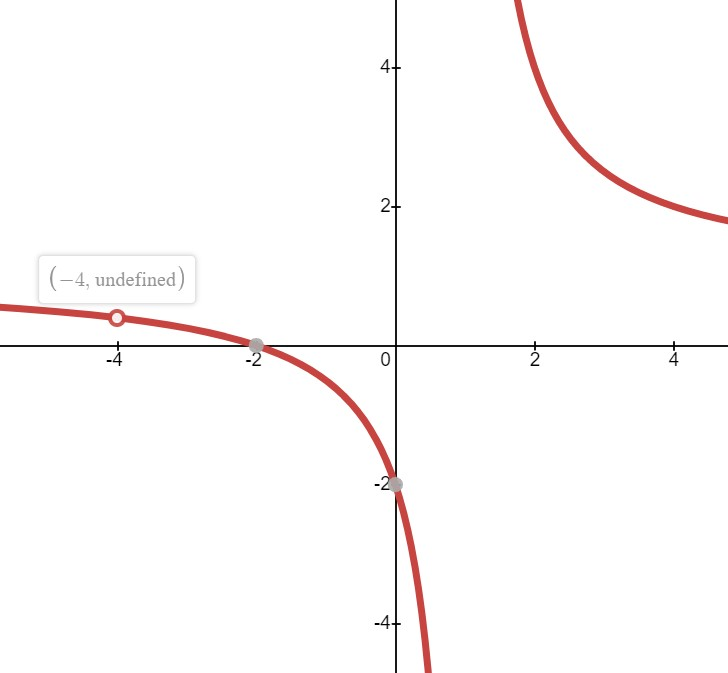
\includegraphics[width=3.5in]{Figures/rational.jpg}
\begin{solution}
  The function \(h(x)\) has a hole because plugging in values near \(-4\) still
  give well-defined numbers and the function gets \emph{arbitrarily}
  close to a real number. In other words, it does not go off to
  \(\infty\) or \(-\infty\). 
\end{solution}
How does the function $k(x)=\displaystyle\frac{x+2}{x-1}$ compare to $h(x)$?
\begin{solution}
  \(h(x)\) is not defined at \(x=-4\), but \(k(-4) = -2/(-5) =
  2/5\). However, \(h(x)\) and \(k(x)\) agree on every other
  value (since \(x^2+3x-4 = (x-1)(x+4)\)). This means we can say \[
    \lim_{x \to -4} \frac{(x+2)(x+4)}{x^2+3x-4} = \lim_{x \to -4}
    \frac{x+2}{x-1} = \frac{2}{5} \,.
  \]
\end{solution}
\pagebreak
%
% Instructor note: they are NOT the same function since their domains are different, but they agree except at -4, which makes sense because when x isn't -4 we can cancel the common factor in h(x)
%

\vspace{-0.1in}
\noindent\fbox{%
	\parbox{\textwidth}{
		\textbf{Limits}: We write $\displaystyle \lim_{x\to c} f(x) = L$ if the values of $f(x)$ approach $L$ as $x$ approaches $c$.
	}%
}
Note that the value of the function \underline{at} $c$ is not
relevant, and does not even need to be defined!

\question Draw the graphs of $f(x) =\displaystyle \frac{x}{x}$ and
$g(x) = \displaystyle \frac{x}{|x|}$ on the board and consider whether each has a limit at 0.
\begin{solution}
  See
  \href{https://www.desmos.com/calculator/hkh1rlx0pk}{https://www.desmos.com/calculator/hkh1rlx0pk}
  for graphs. \[
    \lim_{x\to 0} \frac{x}{x} = 1 \quad\text{ but } \lim_{x \to 0}
    \frac{x}{|x|} \text{ DNE}
  \]
\end{solution}

\question Do these functions have limits at 0?

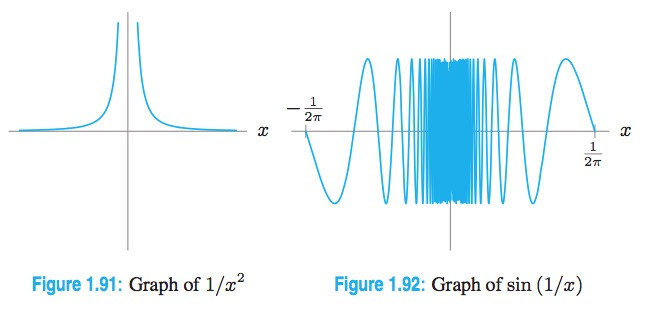
\includegraphics[width=4in]{Figures/nolimits.jpg}



\vspace*{-0.9cm}
\begin{solution}
  No. \(f(x) = \frac{1}{x^2}\) goes off to \(\infty\) has \(x \to 0\),
  but \(\infty\) is not a number, so \(\lim_{x\to 0} \frac{1}{x^2}\)
  DNE. For \(g(x) = \sin(1/x)\), we see that the graph never
  ``settles.'' In other words, as \(x \to 0\), the graph gets
  arbitrarily close to both \(1\) and \(-1\). Thus, \(g(x)\) never
  approaches a single number as \(x\) approaches \(0\), so \(\lim_{x
    \to 0} \sin(1/x)\) DNE.
\end{solution}
\question (1.8 \#1)

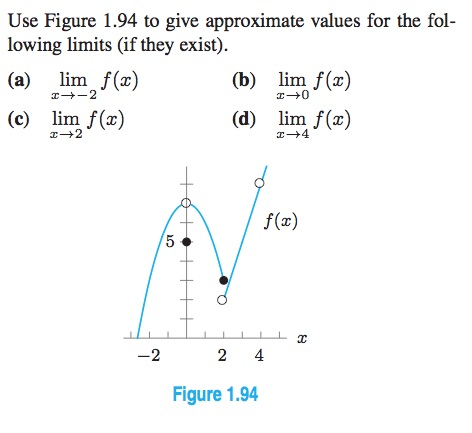
\includegraphics[width=3.5in]{Figures/no1.jpg}

\vspace*{-0.8cm}
\begin{solution}
  \begin{enumerate}
  \item \(\lim_{x\to-2} f(x) \approx 3\)
  \item \(\lim_{x\to 0} f(x) = 7\)
  \item \(\lim_{x \to 2} f(x)\) DNE
  \item \(\lim_{x\to 4} f(x) \approx 8\) 
  \end{enumerate}
\end{solution}
\question Think again about the last problem.  Are there intervals on
which $f$ is not continuous?
\begin{solution}
  \(f(x)\) is not continuous at \(x=0\), \(x=2\), and \(x=4\). We
  cannot see exactly where the domain begins and ends, but \(f(x)\) is
  definitely continuous on \([-2,0) \cup (0,2) \cup (2,4)\).
\end{solution}
Then see if you can finish the definition in the box below.

\noindent\fbox{%
	\parbox{\textwidth}{
		\textbf{Continuity}: The function $f$ is continuous at $c$ if $f$ is defined at $c$ and 
		\ifprintanswers if \[\lim_{x\to c}f(x) = f(c)\,.\]
		\else \vskip8ex\fi
		The function $f$ is continuous on an interval $[a,b]$ if it continuous at every point in the interval.
		
	}%
}
\question Consider the function
$$N(u) =  \left\lbrace \begin{array}{ll} \! \! e + 3^{u^2+k} & \textrm{if } u<1. \\ \!\! 5e \ln \left( e + u -1 \right) & \textrm{if } u \geqslant 1. \end{array}\right.$$
Find all values of k so that $N(u)$ is continuous at $u = 1$. Show your work carefully, and leave your answer(s) in exact form.
\begin{solution}
  With our definition of continuity, we need for \(\lim_{u \to 1} N(u)
  = N(1) = 5e\ln(e+1-1) = 5e\). However, for this to happen, it must
  be that \[
    5e = \lim_{u \to 1} (e+3^{u^2+k}) = e+3^{1+k} \,.
  \]
  Thus, we solve
  \begin{align*}
    e+3^{1+k} = 5e
    & \implies 3^{1+k} = 4e \\
    & \implies 1+k = \log_3(4e) \\
    & \implies k = \log_3(4e)-1
  \end{align*}

\end{solution}
\end{questions}
\ifprintanswers
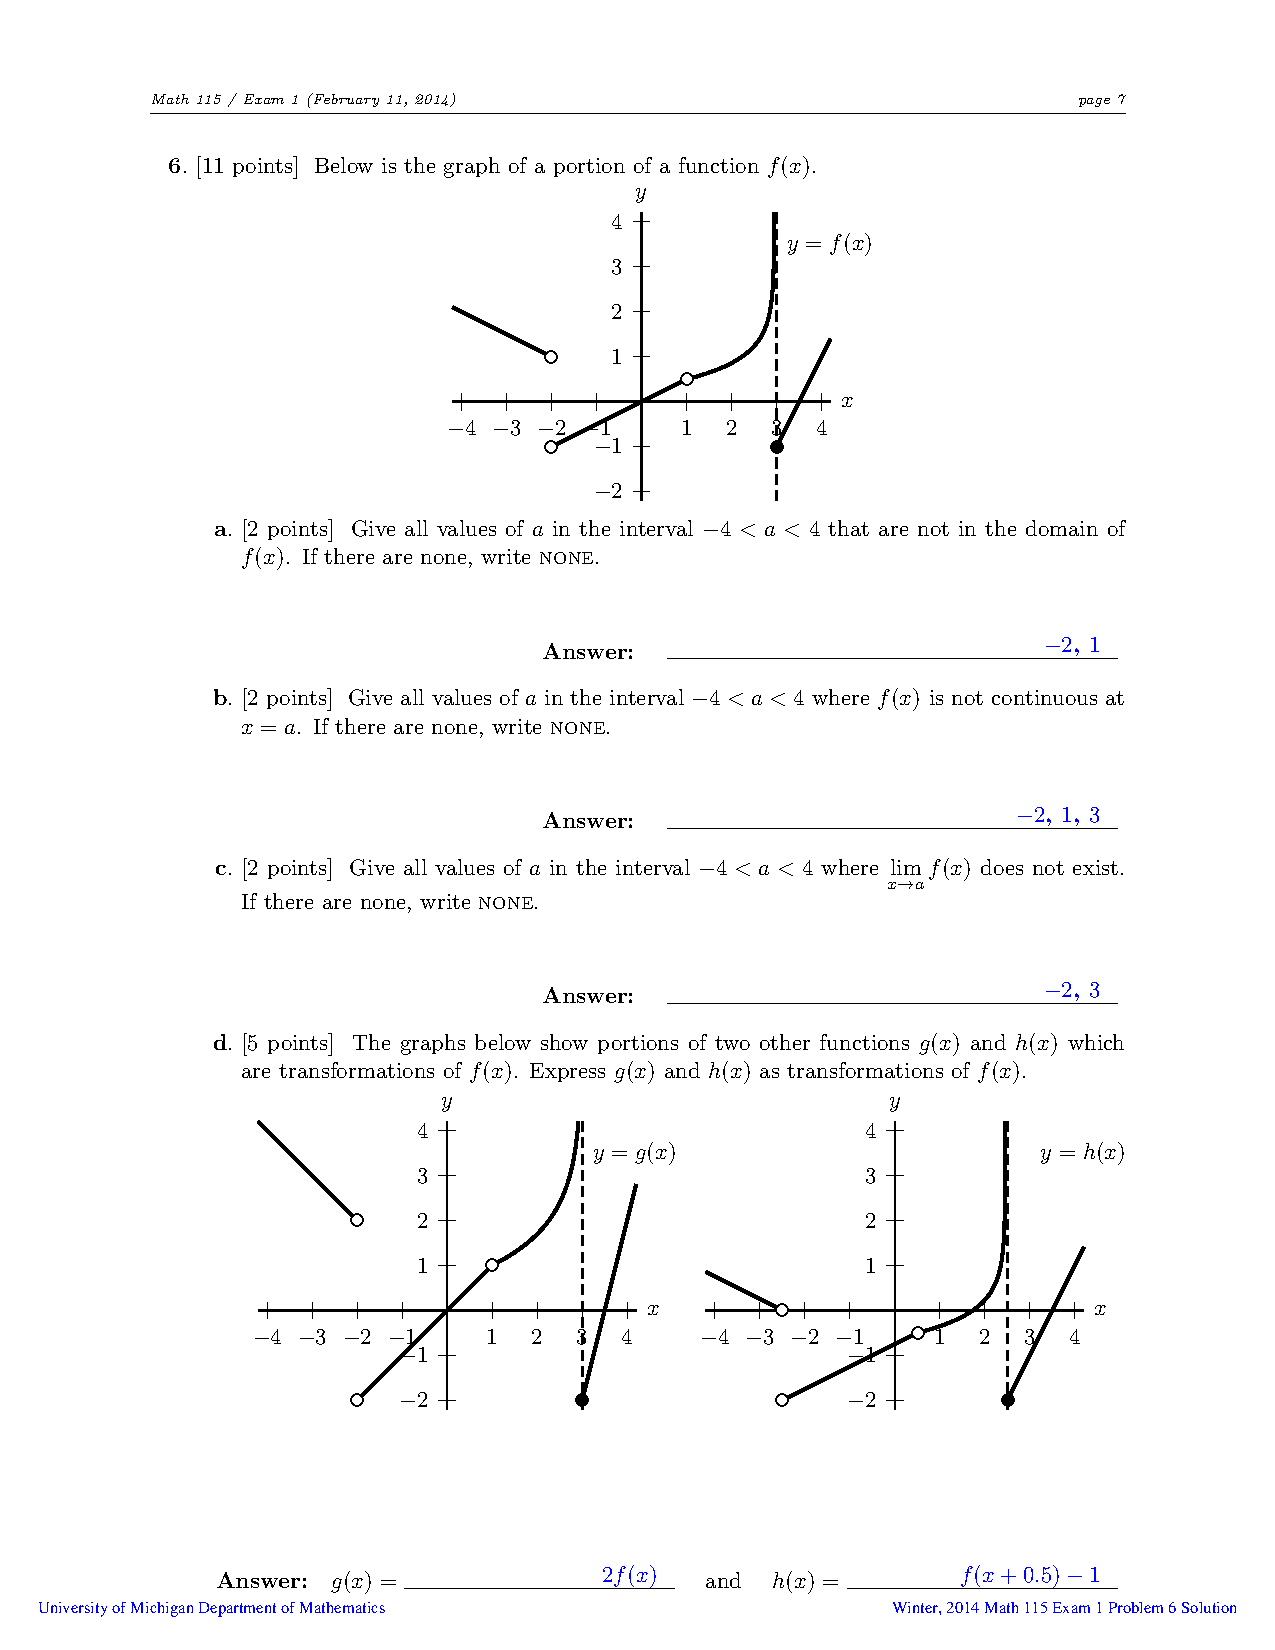
\includepdf[pages=-,pagecommand={\thispagestyle{empty}}]{Figures/s6.pdf}
\else
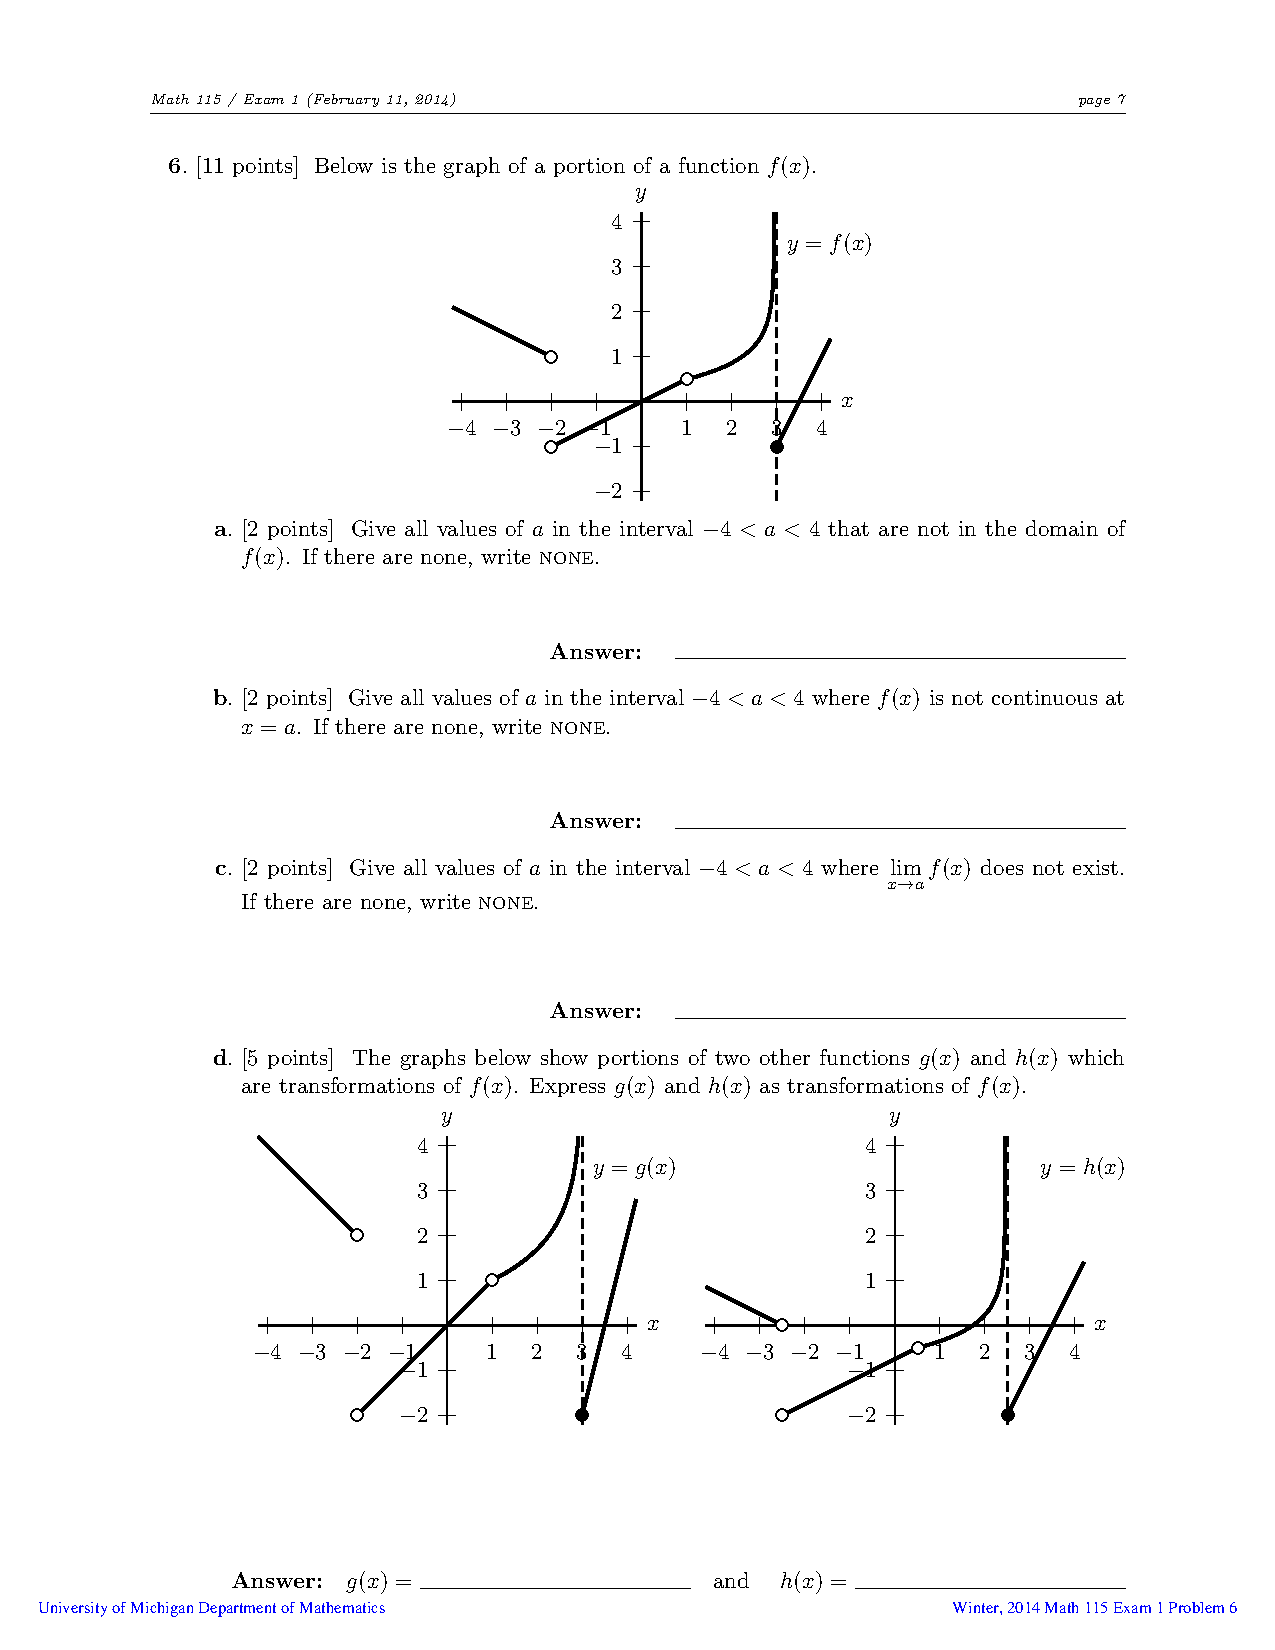
\includepdf[pages=-,pagecommand={\thispagestyle{empty}}]{Figures/p6.pdf}
\fi
\ifprintanswers
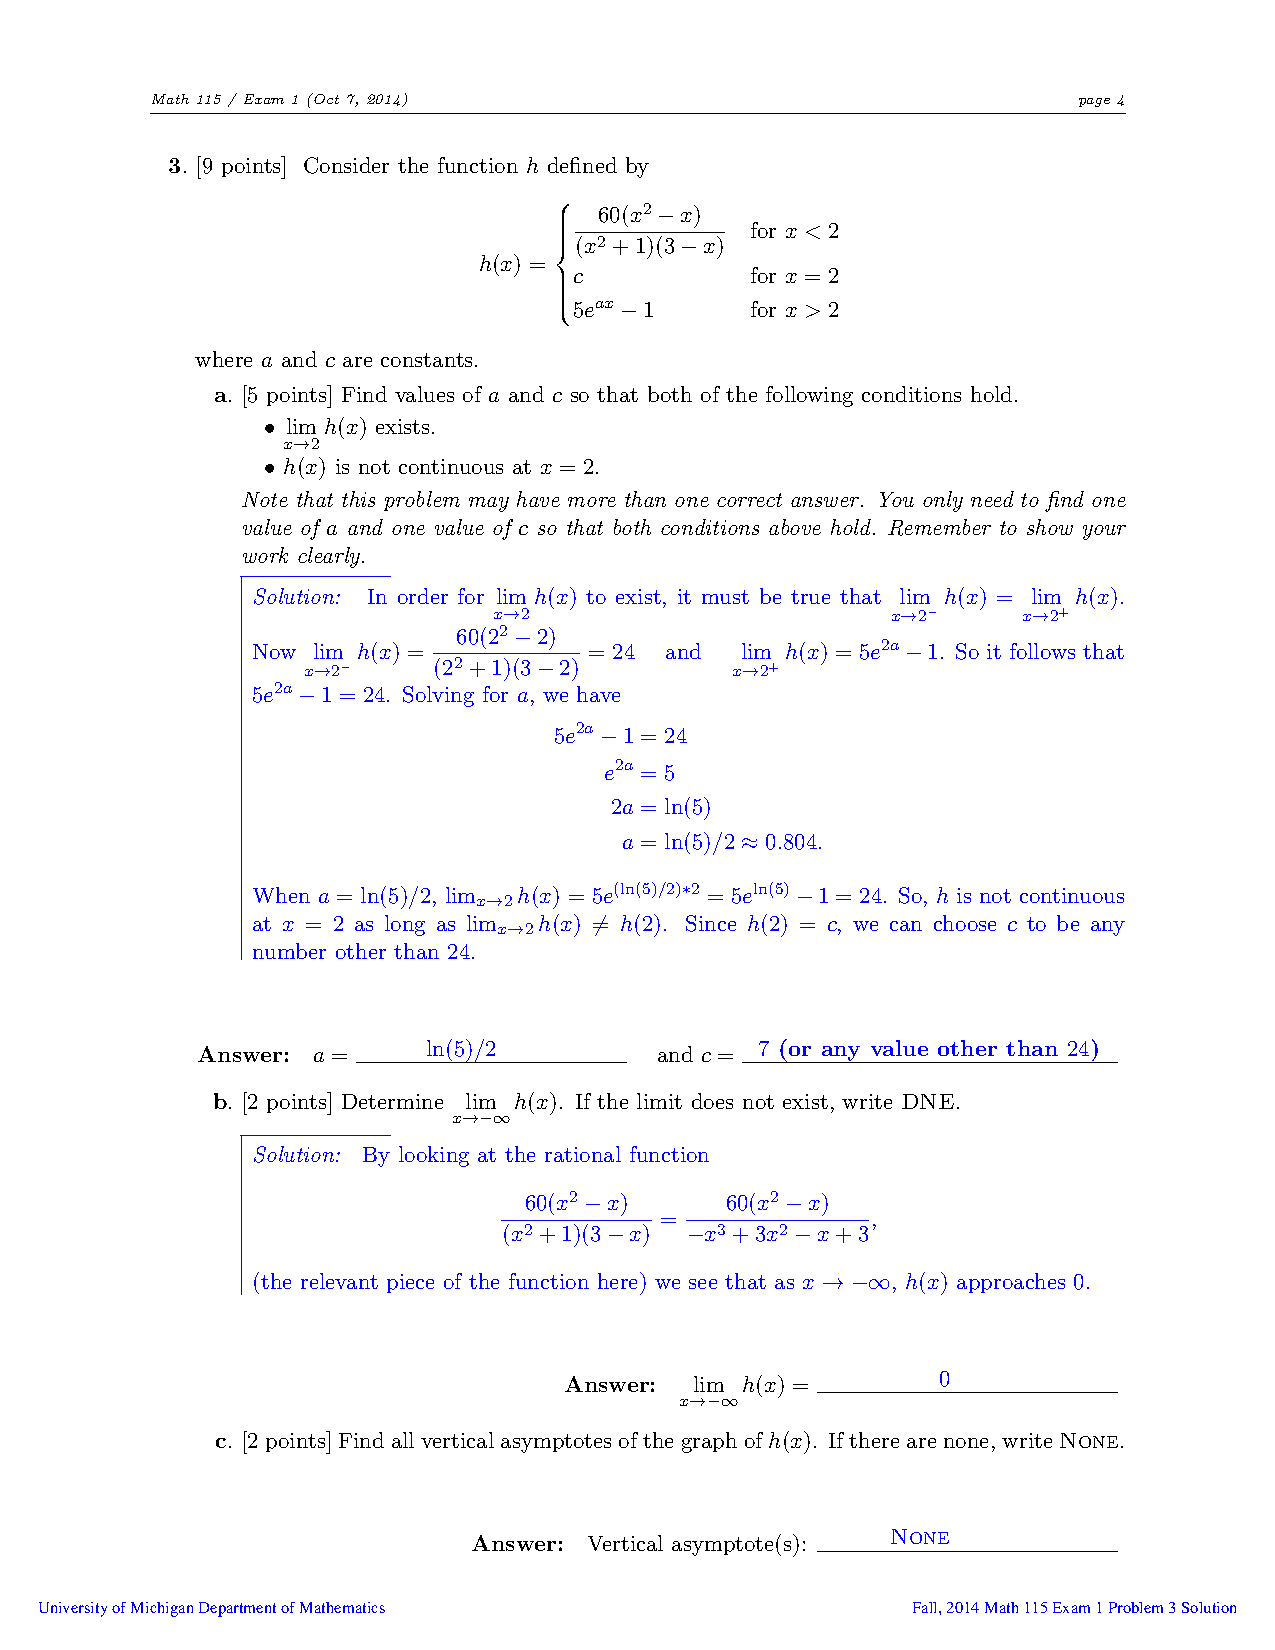
\includepdf[pages=-,pagecommand={\thispagestyle{empty}}]{Figures/s3.pdf}
\else
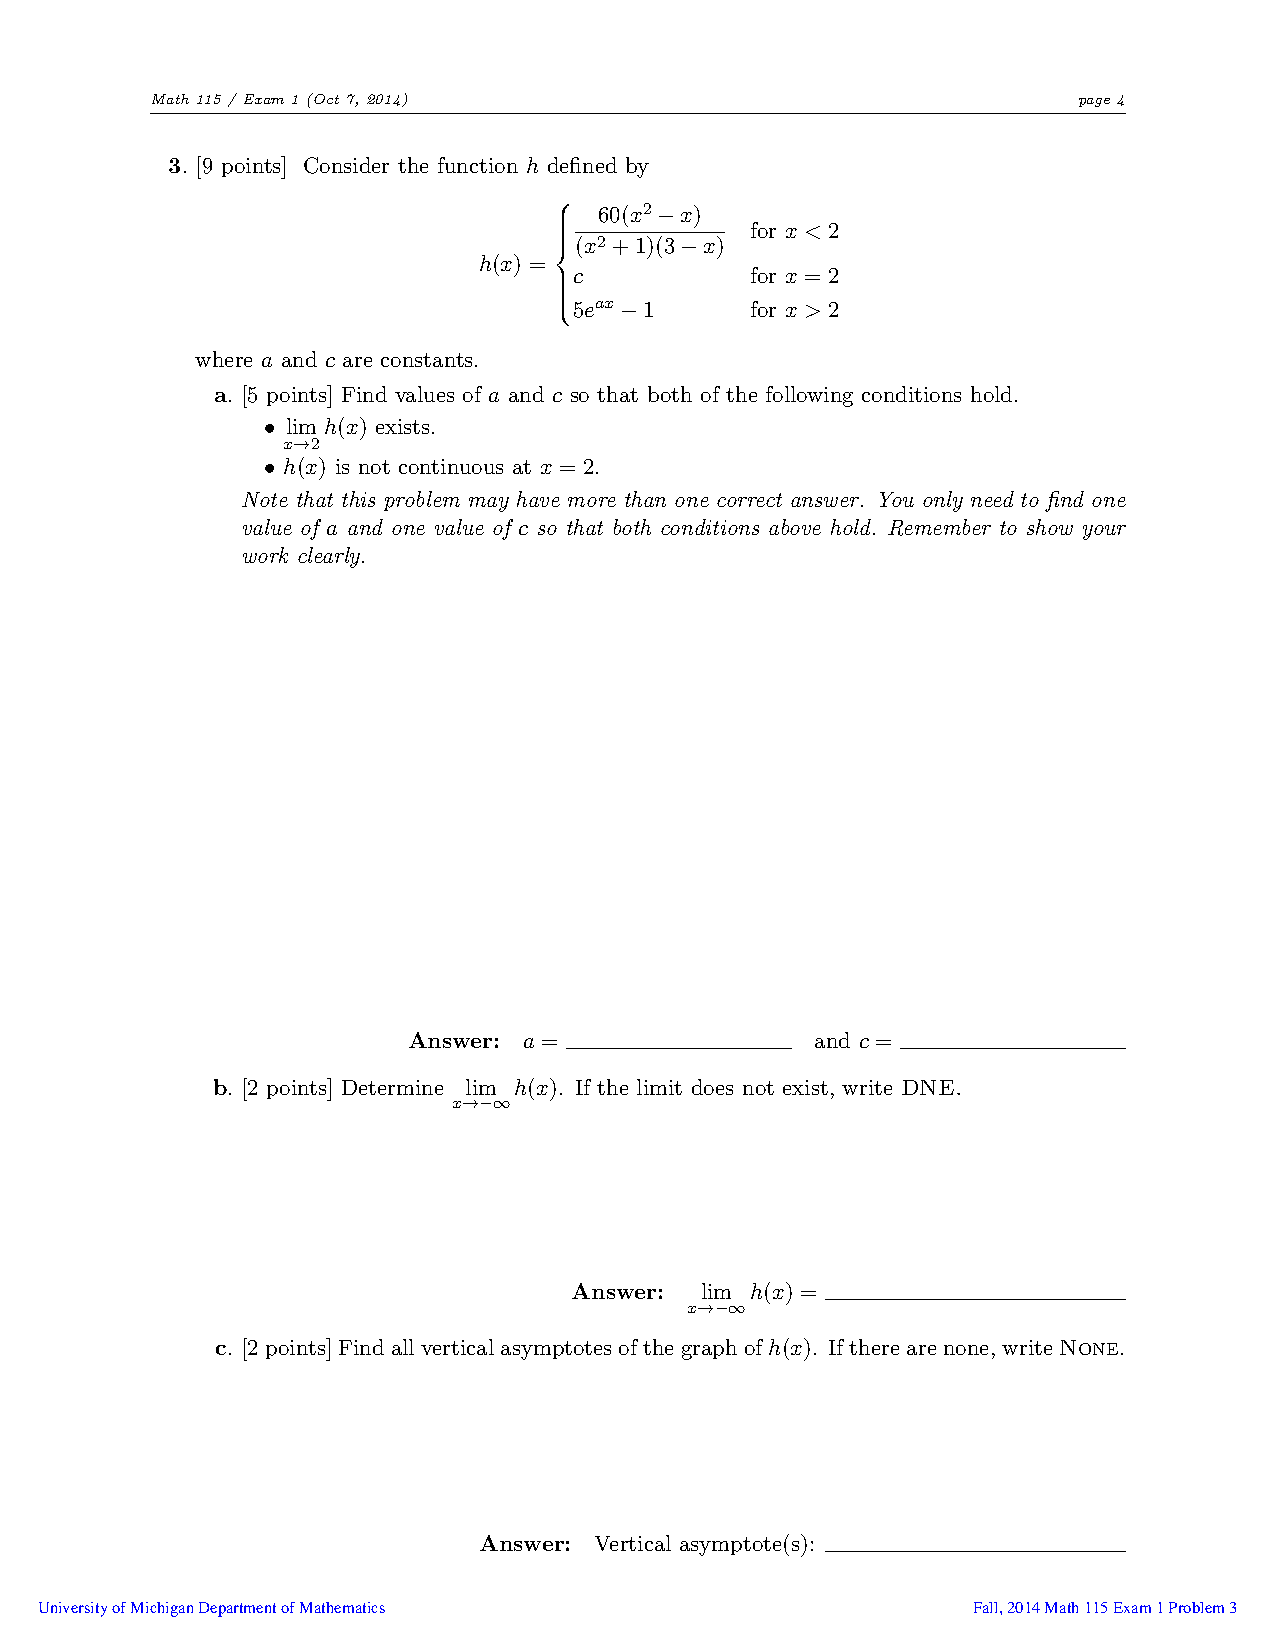
\includepdf[pages=-,pagecommand={\thispagestyle{empty}}]{Figures/p3.pdf}
\fi

\end{document}